\section{Road profiles and forcing}

\begin{frame}[fragile]{Road data as CSV}
  \begin{itemize}
    \item \texttt{draw\_bumpy.csv}: short sample, columns \texttt{x,h}
    \item \texttt{bumpy.csv}: generated file,
          columns \texttt{x,h0,h1,\ldots}
          (several realizations)
  \end{itemize}
  Generate the full file:
\begin{lstlisting}[style=terminal]
uv run python generate_road_profiles.py
uv run python plot_roads.py
\end{lstlisting}
\end{frame}

\begin{frame}{Road profiles}
  \begin{center}
    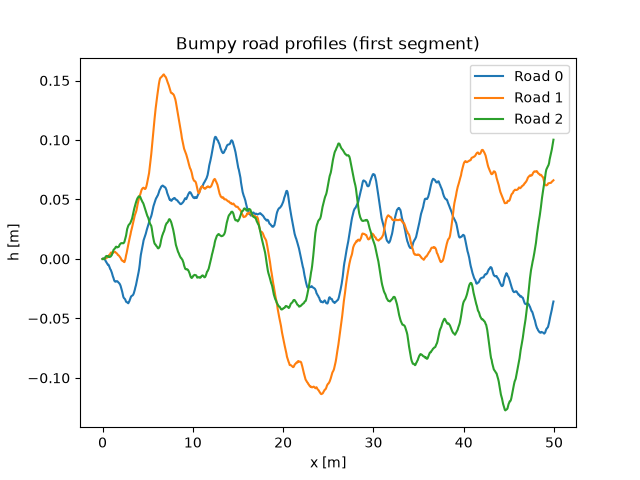
\includegraphics[width=0.70\textwidth]{figures/road_profiles.png}
  \end{center}
\end{frame}

\begin{frame}[fragile]{Loading the CSV}
  \lstinputlisting[style=pythoncompact]{code/load_road_csv.py}
  \begin{itemize}
    \item First column $\to$ distance $x$
    \item Remaining columns $\to$ height profiles
          (rows of \texttt{h\_data})
  \end{itemize}
\end{frame}

\begin{frame}[fragile]{2D array layout (quick reminder)}
\begin{lstlisting}[style=pythoncompact]
>>> h_data.shape          # (nroads, npoints)
(3, 10001)
>>> h = h_data[0, :]      # first road profile
>>> h_data[1, 10:15]      # slice of second profile
\end{lstlisting}
\end{frame}

\begin{frame}{Acceleration from curvature}
  \[
  F(t) \sim -m\, v^2\, h''(x)
  \]
  Approximate $h''(x)$ by centered finite differences on the road mesh.
\end{frame}

\begin{frame}[fragile]{Scalar and vectorized acceleration}
  \lstinputlisting[style=pythonTiny]{code/acceleration.py}
\end{frame}

\begin{frame}[fragile]{Looping over road realizations}
  \lstinputlisting[style=pythoncompact]{code/bumpy_loop.py}
  Resulting list:
  \texttt{[x, t, [h,F,u], [h,F,u], \ldots]}.
\end{frame}
